% !TeX root = ../main.tex

\chapter{动机和背景}
\label{chap:background}

本章将介绍本研究的动机和相关背景。
\autoref{sec:bg-perf-isolation}将介绍SSD资源池化系统中的多组合性能隔离问题重要性,
以及SSD的读写干扰问题及其产生的原因。
\autoref{sec:bg-related-work}将分别从硬盘本身和系统设计的层面介绍改进SSD存储系统服务质量的相关工作。

\section{闪存资源池化系统中的多租户性能隔离问题}
\label{sec:bg-perf-isolation}

现代的虚拟化和资源池化技术使得云系统中的多个租户可以共享同一个物理资源,却给每个租户独占该资源的假象~\cite{bugnion2017hardware}。
在这种抽象中,各个租户间的性能隔离对于满足租户的服务质量要求至关重要~\cite{somani2009isolation}。
若云系统的性能隔离不够充分,则每个租户随时可能受到其“吵闹的邻居”(Noisy Neighbor)的影响,其性能的稳定性将会受损。

在存储系统中,性能隔离主要指的是任一租户对物理资源访问的带宽和延迟基本不受其他租户的影响。
由于机械硬盘的延迟普遍较差,且读写性能差异不大,因此限制各个租户的带宽往往就可以实现多租户的性能隔离。
例如,Docker通过Linux的cgroup~\cite{cgroup}设置每个租户的带宽上限;
Ceph~\cite{weil2006ceph}也通过mClock~\cite{gulati2010mclock}实现分布式的租户资源限制。
\JF{怎么实现的?}

然而,交互性高的数据应用服务需要良好的存储尾延迟保证~\cite{dean2013tail,hao2016tail}。
例如,某些用户除了对访问带宽有要求,还会要求对自己租用的SSD的读请求中99\%均有两毫秒以下的延迟。
尽管可以通过设置不同租户的优先级保证某些租户的请求被优先服务,但并不能给出严格的尾延迟保证。
在这种情况下,仅仅对每个用户的访问带宽进行限制是不够的。

\begin{figure}[h]
  \centering
  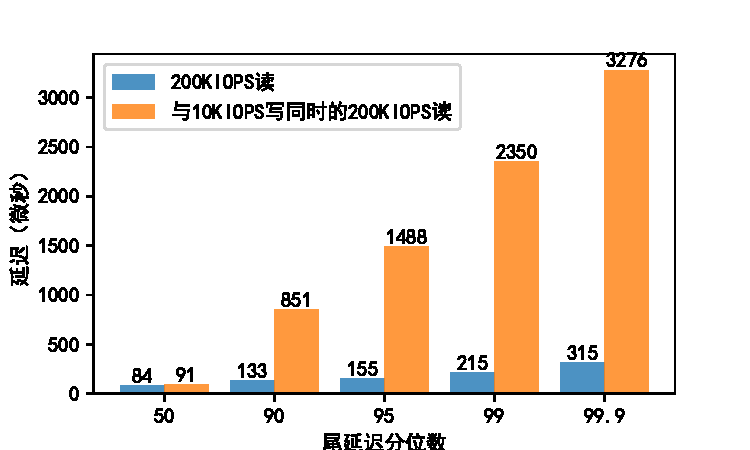
\includegraphics[width=0.8\textwidth]{thesis-wr-interfere.pdf}
  \caption{写操作对其他租户读延迟的影响}
  \label{fig:bg-wr-interfere}
\end{figure}

SSD内部的\textit{读写干扰}使多租户的性能隔离更加复杂。
如\autoref{fig:bg-wr-interfere}所示,当一个租户在进行读操作时,另一个租户对不同位置的写操作是该租户的尾延迟增大了约十倍。
这是由于写操作触发的SSD内部的垃圾回收、缓冲区刷新等行为引起的。
为了取得良好的性能,SSD内部的存储采用日志结构~\cite{ArpaciDusseau18-Book},
逻辑地址进行转换后才得到真正的物理地址,所以资源池化系统对多个租户的逻辑存储空间进行的划分不能阻止多个租户的数据被存放在一起。
当某个租户进行写操作时,SSD内部可能会进行针对某一区域的垃圾回收或缓冲区刷新,使得该硬盘上其他租户的访问性能受到影响。

\section{相关工作}
\label{sec:bg-related-work}

\subsection{保证服务质量的SSD}

从SSD本身来设计(灰盒SSD)。

获取SSD内部信息,SSD性能建模(加Linnos)。

\subsection{保证服务质量的云服务系统}

老方法:cgroup,bfq,mclock?后续?不写了?

新方法:redundancy、各种Job Scheduler